\chapter{Neural Networking Technology}

\label{ch:background} 

%Explaining what your project does that is new or is better than existing work in the same field.
Neural networking is a technique that mimics biological intelligence in order to
create artificially intelligent systems. Development of this technology has given the
computer science community great leverage in helping machines to emulate human
beings and intelligent animals. While the underlying concepts of neural networking have
been around for some time, modern refinements to the technology and its application
have spurred renewed interest in advancing the science. The combination of neural
networks with modern equipment and techniques paves the way for machines that truly
utilize strong artificial intelligence. This chapter will discuss what new technologies
facilitate neur al networks, and what neural networks mean for the development of
artificial intelligence systems.
\section{What is Neural Networking?}
Neural networks are collections of mathematical models designed to work
together to emulate the known properties of biological nervous systems \cite{three}.
The mammalian brain contains billions of neurons. Thus, although the concept of neural
networking has been around since the 1950s, only recently has the computing power
become available to begin developing true, usable neural networks.\\
Animal brains, including the human brain, comprise massive parallel systems.
That is to say that they process multiple pieces of information at one time. Biological
brains are composed of neurons, which are the interconnected but independent
workhorses of

\begin{figure}
    \centering
    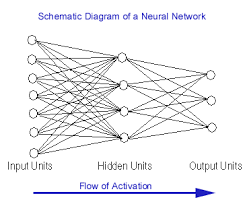
\includegraphics{images/neural.png}
    \caption{Neural Network}
    \source{Source: https://www.innoarchitech.com/artificial-intelligence-deep-learning-neural-networks-explained/}
    \label{fig:my_label}
\end{figure}

biological nervous systems. Each neuron may be connected with as many
as a thousand or more other neurons. This allows mammals to quickly perform tasks like recognizing patterns and faces. For many years, the parallel processing concept kept
computers from effectively emulating these brain functions in the same way. Modern
computer architecture provides several solutions to this problem.
\subsection{The Modern Supercomputer}
Moore’s Law has been amazingly accurate during the lifecycle of the modern
computer. Supercomputers are capable of performing one billion or more operations per
second. These computers in particular were key to the development of early functional
neural networks.\\
The basic electronic computational method, sequential computing, involves the
processing of one piece of information at a time. This piece of information could be as
small as one bit, which has a value of either one or zero. In a black and white picture, it
takes two bits to represent one pixel, or a small dot in the picture. The complexity of
such a picture, called the resolution, is directly related to, and defined by, the number of
pixels representing the picture. A printed page, for example, will often have a resolution
of 300 dots per inch. This means that one square inch of print could be defined by as
many as 90,000 dots, or bits. A simple computer must go through at least 180,000
operations just to process one square inch of printed paper.\\
There have been many tricks employed to help computers deal with this kind of
processing, such as reducing the resolution of pictures being analyzed. Critical
information can often be preserved even when resolution is decreased. But this does not
reach the root of the problem, namely that human beings are somehow capable of
processing printed pages in their native format, and at resolutions even greater than 300
dots per inch. People can quickly scan through entire pages to search for a pattern. Often this pattern will appear to jump off the page and grab the attention of the reader, without
their having to read the entire text. This is the advantage of parallelism, and this is where
computers have traditionally fallen short.\\
Information is processed in some computers in terms bytes or vectors, which are
collections of bits. A vector may contain 100 to 1000 bits or even more. These are still,
however, only small scalar multiples in terms of processing power. Even if a computer
processed 100 bits simultaneously, it would still require 168,300 operations just to read in
a standard 8 ½ x 11 inch piece of paper. Whereas people might skip right over white
space, a computer must analyze every square inch in order to make sure that it is actually
white space. Actual processing of the information could also take thousands or tens of
thousands of operations per bit to analyze its relationship with neighboring bits. Since
human beings and other animals see much more than an 8 ½ x 11 inch window, it
becomes clear that supercomputers are necessary to emulate neural processing in a
sequential environment.
\subsection{Parallel Computing and Distributed Networks}
It is much faster to work with multiple pieces of information if they can all be
processed at the same time. This is called parallel processing. The beginnings of
parallelism in computing are represented by the vector-based computing architecture
discussed above. Parallel processing used to be infeasible for general use because
hardware was at such a premium. It is time that is at a premium today, particularly
human time. The addition of a processor in a computer may cost only a few hundred
dollars, and may bring an increase in speed of 85\%. Assuming no human cost to parallelize the task, one 50-hour job turned into a 30- hour job recovers the cost of
hardware.\\
Parallel computing can be much more than a pair of processors, however. The
University of Virginia has several projects that are advancing the technology of parallel
computing. Two projects in particular, Legion and Centurion, represent great advances
in building working neural networks.\\
The Centurion project features 384 individual processors connected together and
working in parallel. These processors could combine for up to 240 billion operations per
second, making short work of processing a printed page [Centurion]. The even more
ambitious Legion project is a software system that aims to connect millions of computers
together to work in parallel. The infrastructure that could make this goal a reality is
already built and being refined in the form of the Internet. With tens of millions of
computers simultaneously simulating small neural systems, we could be very close to
fully simulating the estimated 100 billion neurons that comprise the human brain.
Current technology would require a few hundred million computers working in parallel to
accomplish this task.

\section{Implications of Neural Nets on AI}
Certainly, neural networking enhances the possibility of developing intelligent
systems. It is, after all, a direct emulation of what AI programmers are trying to achieve.
In its own way, it solves the previously discussed problem of trying to figure out what it
means for machines to be intelligent. If we consider ourselves intelligent, and directly
emulate our own brains, then the product should likewise be intelligent. The pursuit of intelligent software is neither unsavory nor unethical. Indeed, many perceived
shortcomings in today’s software come in part from our inability to program sufficiently
intelligent programs.\\
Neural networks are already being used successfully in many commercial
applications ranging from document processing to the food industry. Neural network
systems are particularly good at pattern recognition, which has uses in odor analysis,
handwriting recognition, credit analysis and many other tasks. Computers that
are able to do these tasks are useful because, although people are very good at pattern
recognition, we are not as good at the mundane tasks that follow. It is easy, for example,
for a computer to track and analyze credit card use for thousands of people 24 hours a
day. Computers can consistently analyze food odors and aromas in cases where human
sensation may become numb, or in cases where the smell of bad food might make people
sick.\\
Neural networks also bring us closer to developing strong artificial intelligence.
By directly emulating mammalian brains, we should be getting closer to developing a
program that has its own intelligence. If, as is commonly accepted, the entirety of human
intelligence lies within the structure of the brain, it is possible that we need only simulate
enough neurons to mimic that brain. In some ways, we are restricted by our limited
knowledge of actual neural function, but we have substantial observational information
regarding the function of individual neurons [Clabaugh]. With continued research, we
may be able to develop an entire artificial brain.\\

\begin{figure}[H]
    \centering
    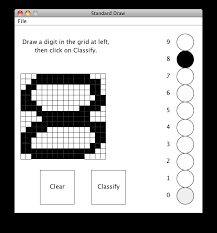
\includegraphics{images/hand.png}
    \caption{Handwriting Recognition}
    \source{Source: https://www.eeweb.com/articles/artificial-intelligence-based-handwriting-recognition}
    \label{fig:my_label}
\end{figure}

The idea of neural networking again raises moral and philosophical
complications. It reintroduces the idea of a living electronic entity in a way that is easier to relate to as human beings. A neural network is a replica (albeit a small and grossly
simplified replica, given current technology) of our own brain structure. Of particular
note in considering moral implications is the fragility of electronic computing systems.
Computers get turned on and off constantly, and in the future we mightn’t need
specialized computer hardware to build complex (human- like) neural networks. The
accidental powering down of a personal computer containing a living entity could happen
in an instant, and would no doubt be morally catastrophic.\\
The ongoing development of modern computing technologies enable
programmers and biologists to simulate real biological systems with increasing accuracy.
Super fast computers and those that process data in parallel help unlock the secrets of
biological nervous systems. But such simulations could mean serious moral
ramifications if they are successful in achieving their goal. Furthermore, the results of
simulating biological life could be more than just theoretical. It is important for
engineers to consider the very likely prospect of (desirable and undesirable) side-effects
from the development of technologies discussed above.

%Test citation \cite{cormen2009introduction}.




















